\documentclass{article}
\usepackage[utf8]{inputenc}
\usepackage{hyperref}
\usepackage{listings}
\usepackage{xcolor}
\usepackage[margin=1in]{geometry}
\usepackage{tikz}
\usepackage{booktabs}
\usepackage{longtable}
\usepackage{array}
\usepackage{enumitem}
\usepackage{fancyhdr}
\usepackage{amsmath}
\usepackage{graphicx}
\usetikzlibrary{shapes.geometric, arrows.meta, positioning, calc}

% --- Colour palette ------------------------------------------------------------
\definecolor{codegreen}{rgb}{0,0.6,0}
\definecolor{codegray}{rgb}{0.5,0.5,0.5}
\definecolor{codepurple}{rgb}{0.58,0,0.82}
\definecolor{backcolour}{rgb}{0.95,0.95,0.92}
\definecolor{evblue}{RGB}{30,100,200}
\definecolor{emsgreen}{RGB}{20,140,80}
\definecolor{cargoamber}{RGB}{200,120,0}
\definecolor{stmred}{RGB}{180,30,30}

% --- Listing style -------------------------------------------------------------
\lstdefinestyle{mystyle}{
    backgroundcolor=\color{backcolour},
    commentstyle=\color{codegreen},
    keywordstyle=\color{magenta},
    numberstyle=\tiny\color{codegray},
    stringstyle=\color{codepurple},
    basicstyle=\ttfamily\footnotesize,
    breakatwhitespace=false,
    breaklines=true,
    captionpos=b,
    keepspaces=true,
    numbers=left,
    numbersep=5pt,
    showspaces=false,
    showstringspaces=false,
    showtabs=false,
    tabsize=2,
}
\lstdefinelanguage{json}{
    morestring=[b]",
    morecomment=[l]{//},
    sensitive=false,
}
\lstset{style=mystyle}

% --- Page header ---------------------------------------------------------------
\pagestyle{fancy}
\fancyhf{}
\rhead{SIAM EV Platform --- Truck Device Protocol}
\lhead{\leftmark}
\rfoot{Page \thepage}
\renewcommand{\headrulewidth}{0.4pt}

\hypersetup{
    colorlinks=true,
    linkcolor=evblue,
    urlcolor=evblue,
    pdftitle={Truck Device Communication Protocol},
    pdfauthor={Ruslee Sutthaweekul}
}

% --- Document ------------------------------------------------------------------
\title{%
    \textbf{SIAM EV Platform}\\[6pt]
    \large Truck Device Communication Protocol\\[4pt]
    \normalsize STM32H7 $\cdot$ GPS $\cdot$ OBD-II $\cdot$ Dual Camera $\cdot$ 3G/4G
}
\author{Ruslee Sutthaweekul}
\date{Version 1.0 \quad\textbullet\quad \today}

\begin{document}

\maketitle
\tableofcontents
\newpage

% ==============================================================================
\section{Overview}
% ==============================================================================

This document specifies the communication protocol between the on-board truck
monitoring unit (TMU) and the SIAM EV cargo monitoring backend. It covers
message formats, transport configuration, security, and the firmware state
machine required to implement correct behaviour on the STM32H7 controller.

\subsection{Hardware Summary}

\begin{center}
\begin{tabular}{lll}
\toprule
\textbf{Component} & \textbf{Physical interface to MCU} & \textbf{Role}\\
\midrule
MCU              & STM32H7 series        & Main controller; runs full protocol and TLS stack\\
Camera 1         & SPI-Eth Module 1      & Generic IP camera, cargo front; HTTP snapshot\\
Camera 2         & SPI-Eth Module 2      & Generic IP camera, cargo rear; HTTP snapshot\\
GPS              & UART (NMEA 0183)      & Position, speed, heading; primary clock source\\
OBD-II           & CAN bus (ISO 15765-4) & Vehicle bus: speed, RPM, fuel, fault codes\\
3G/4G module     & UART (AT commands)    & Internet uplink; controlled entirely by STM32H7\\
SPI-Eth Module 1 & SPI                   & Ethernet interface for Camera 1 (e.g.\ W5500)\\
SPI-Eth Module 2 & SPI                   & Ethernet interface for Camera 2 (e.g.\ W5500)\\
\bottomrule
\end{tabular}
\end{center}

\subsection{On-Board Connectivity}

Each IP camera has a dedicated SPI-Ethernet module (e.g.\ Wiznet W5500)
providing an isolated Ethernet segment. There is no shared switch. The 3G/4G
module is a UART peripheral --- it is not a router and has no IP address on
any truck LAN. The STM32H7 is the only device with internet access; it
manages the cellular link entirely via AT commands and runs TLS in firmware.

\begin{center}
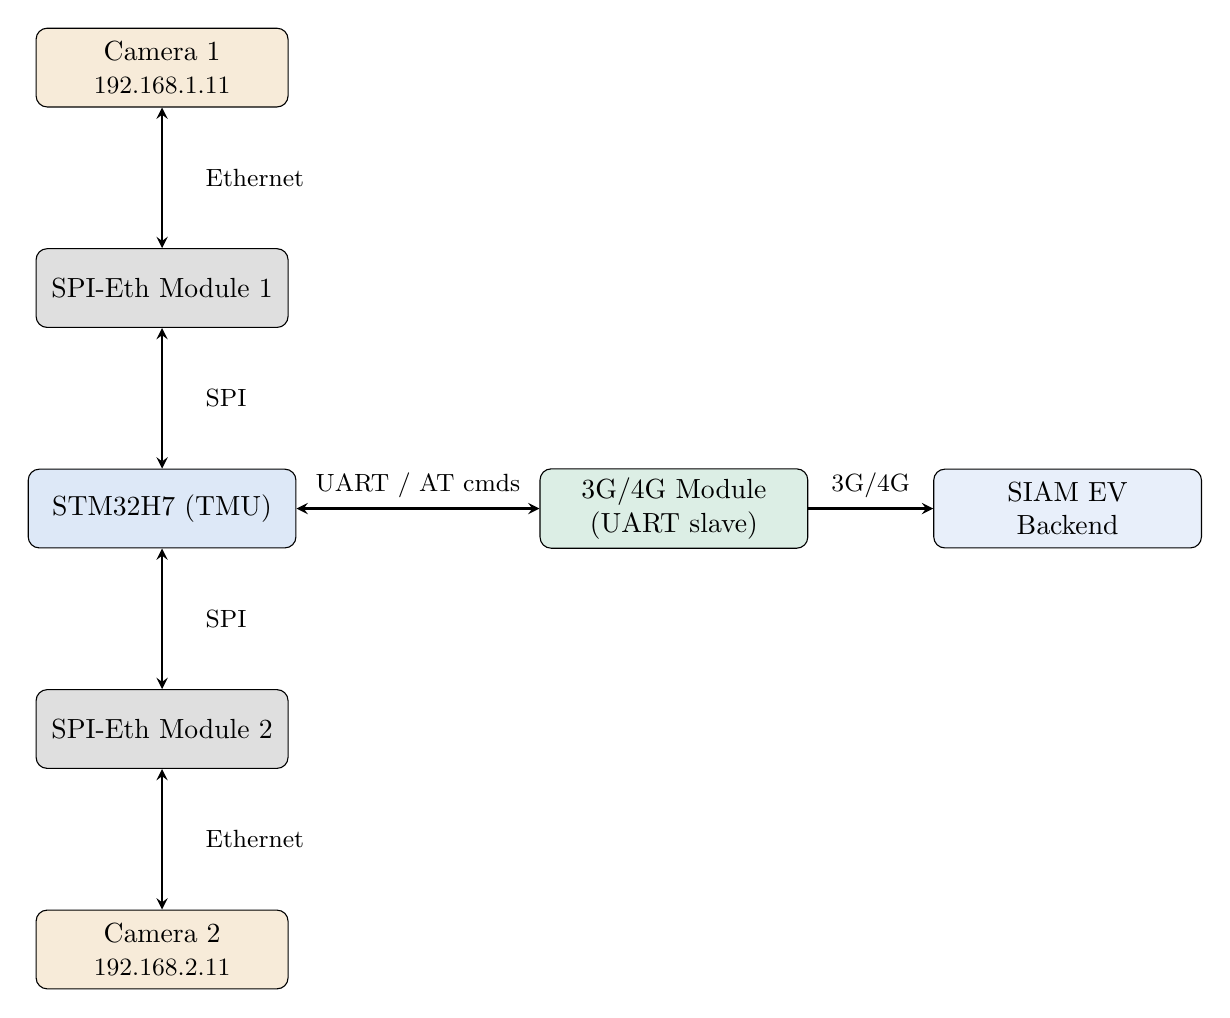
\begin{tikzpicture}[
    box/.style={rectangle, rounded corners, draw, minimum width=3.2cm,
                minimum height=1.0cm, text centered, align=center, fill=gray!10},
    arrow/.style={thick,->,>=stealth},
    darrow/.style={thick,<->,>=stealth}]

% Vertical stack -- 2.8 cm between centres so labels sit clearly in the gap
\node (cam1)    [box, fill=cargoamber!15]                   at (0,  8.4) {Camera 1\\{\small 192.168.1.11}};
\node (spieth1) [box, fill=gray!25]                         at (0,  5.6) {SPI-Eth Module 1};
\node (stm)     [box, fill=evblue!15, minimum width=3.4cm] at (0,  2.8) {STM32H7 (TMU)};
\node (spieth2) [box, fill=gray!25]                         at (0,  0.0) {SPI-Eth Module 2};
\node (cam2)    [box, fill=cargoamber!15]                   at (0, -2.8) {Camera 2\\{\small 192.168.2.11}};

% Right side (horizontal, aligned with STM32H7)
\node (modem) [box, fill=emsgreen!15, minimum width=3.4cm] at (6.5, 2.8) {3G/4G Module\\(UART slave)};
\node (cloud) [box, fill=evblue!10,   minimum width=3.4cm] at (11.5, 2.8){SIAM EV\\Backend};

% Vertical connections -- label right of the line, centred in the gap
\draw [darrow] (cam1)    -- node[right=12pt, font=\small]{Ethernet} (spieth1);
\draw [darrow] (spieth1) -- node[right=12pt, font=\small]{SPI}      (stm);
\draw [darrow] (stm)     -- node[right=12pt, font=\small]{SPI}      (spieth2);
\draw [darrow] (spieth2) -- node[right=12pt, font=\small]{Ethernet} (cam2);

% Horizontal connections
\draw [darrow] (stm)   -- node[above, font=\small]{UART / AT cmds} (modem);
\draw [arrow]  (modem) -- node[above, font=\small]{3G/4G}           (cloud);

\end{tikzpicture}
\end{center}

\begin{center}
\begin{tabular}{lll}
\toprule
\textbf{Device} & \textbf{IP address} & \textbf{Notes}\\
\midrule
STM32H7 (via SPI-Eth 1) & 192.168.1.10 & eth0; Camera 1 network\\
Camera 1 (front)        & 192.168.1.11 & Snapshot endpoint: \texttt{/snapshot.jpg}\\
STM32H7 (via SPI-Eth 2) & 192.168.2.10 & eth1; Camera 2 network\\
Camera 2 (rear)         & 192.168.2.11 & Snapshot endpoint: \texttt{/snapshot.jpg}\\
3G/4G module            & n/a          & UART peripheral; no IP address\\
\bottomrule
\end{tabular}
\end{center}

\noindent Camera snapshot URL (HTTP GET, point-to-point Ethernet):
\begin{lstlisting}[language=bash]
http://192.168.1.11/snapshot.jpg     # Camera 1 -- cargo front (SPI-Eth 1)
http://192.168.2.11/snapshot.jpg     # Camera 2 -- cargo rear  (SPI-Eth 2)
\end{lstlisting}

If a camera requires HTTP Basic Auth, credentials are stored in STM32H7
protected flash and never transmitted off the truck.

% ==============================================================================
\subsection{Hardware Block Diagram}
\label{sec:hw-diagram}
% ==============================================================================

Figure~\ref{fig:hw-wiring} shows the physical signal buses connecting all
on-board components. Power rails are shown in orange dashed lines; all
signal buses are solid bidirectional arrows.

\begin{figure}[h]
\centering
\resizebox{\textwidth}{!}{%
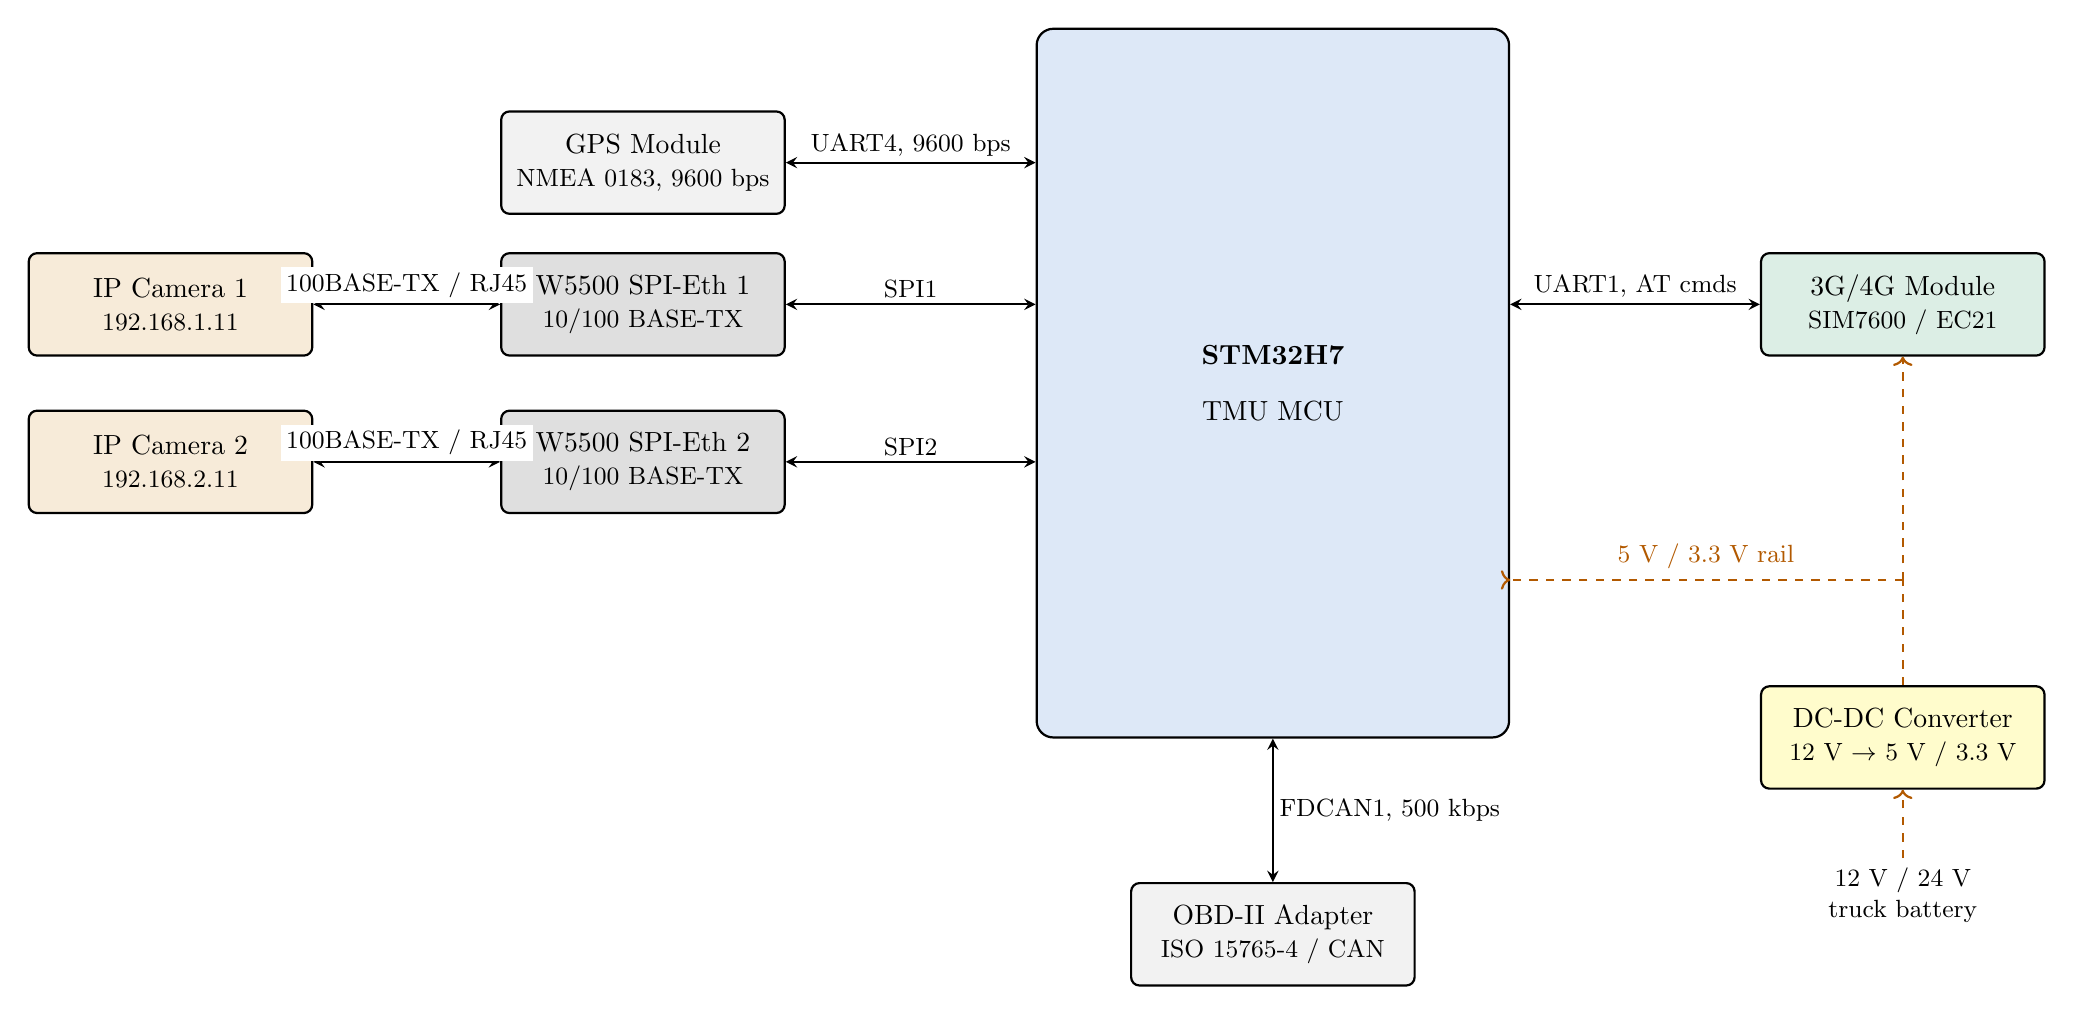
\begin{tikzpicture}[
    periph/.style={rectangle, rounded corners=3pt, draw, thick,
                   minimum width=3.6cm, minimum height=1.3cm,
                   text centered, align=center, fill=gray!10},
    bus/.style={thick, <->, >=stealth},
    pwr/.style={thick, dashed, orange!70!black},
    lbl/.style={font=\small, fill=white, inner sep=2pt}]

%% ── Central MCU ──────────────────────────────────────────────────────────────
\node[draw, thick, rounded corners=6pt, fill=evblue!15,
      minimum width=6cm, minimum height=9cm, align=center] (mcu) at (0,0)
    {\textbf{STM32H7}\\[8pt]{\normalsize TMU MCU}};

%% ── Peripherals ──────────────────────────────────────────────────────────────
%% Left column
\node[periph] (gps) at (-8, 2.8)
    {GPS Module\\{\small NMEA 0183, 9600 bps}};

\node[periph, fill=gray!25] (spieth1) at (-8, 1.0)
    {W5500 SPI-Eth 1\\{\small 10/100 BASE-TX}};

\node[periph, fill=gray!25] (spieth2) at (-8,-1.0)
    {W5500 SPI-Eth 2\\{\small 10/100 BASE-TX}};

%% Far left (cameras)
\node[periph, fill=cargoamber!15] (cam1) at (-14, 1.0)
    {IP Camera 1\\{\small 192.168.1.11}};

\node[periph, fill=cargoamber!15] (cam2) at (-14,-1.0)
    {IP Camera 2\\{\small 192.168.2.11}};

%% Right column
\node[periph, fill=emsgreen!15] (modem) at (8, 1.0)
    {3G/4G Module\\{\small SIM7600 / EC21}};

%% Bottom
\node[periph] (obd) at (0,-7)
    {OBD-II Adapter\\{\small ISO 15765-4 / CAN}};

%% Power
\node[periph, fill=yellow!20] (pwr) at (8,-4.5)
    {DC-DC Converter\\{\small 12 V $\rightarrow$ 5 V / 3.3 V}};

%% ── Signal connections ───────────────────────────────────────────────────────
\draw[bus] (gps.east)
    -- node[lbl, above]{UART4, 9600 bps}
    (mcu.west |- gps);

\draw[bus] (spieth1.east)
    -- node[lbl, above]{SPI1}
    (mcu.west |- spieth1);

\draw[bus] (spieth2.east)
    -- node[lbl, above]{SPI2}
    (mcu.west |- spieth2);

\draw[bus] (cam1.east)
    -- node[lbl, above]{100BASE-TX / RJ45}
    (spieth1.west);

\draw[bus] (cam2.east)
    -- node[lbl, above]{100BASE-TX / RJ45}
    (spieth2.west);

\draw[bus] (mcu.east |- modem)
    -- node[lbl, above]{UART1, AT cmds}
    (modem.west);

\draw[bus] (mcu.south)
    -- node[lbl, right]{FDCAN1, 500 kbps}
    (obd.north);

%% ── Power chain ──────────────────────────────────────────────────────────────
%% Truck 12V source
\node[font=\small, align=center] (bat) at (8,-6.5) {12 V / 24 V\\truck battery};
\draw[pwr, ->] (bat.north) -- (pwr.south);

%% DC-DC to modem (vertical up)
\draw[pwr] (pwr.north) -- (8, -2.5);
\draw[pwr, ->] (8,-2.5) -- (modem.south);

%% DC-DC to MCU (L-shape: right column up then left into MCU)
\draw[pwr] (8,-2.5) -- (3,-2.5);
\draw[pwr, ->] (3,-2.5) -- (mcu.east |- 0,-2.5);

\node[font=\small, text=orange!70!black] at (5.5,-2.2) {5 V / 3.3 V rail};

\end{tikzpicture}%
}
\caption{Hardware block diagram. Black: signal buses. Orange dashed: power chain.}
\label{fig:hw-wiring}
\end{figure}

\subsection{3G/4G Module Interface}
\label{sec:modem-interface}

The cellular module (e.g.\ Quectel EC21/EC25, SIM7600, u-blox SARA-R4) is
treated as a byte-pipe peripheral. The STM32H7 firmware:

\begin{enumerate}[leftmargin=*, label=\arabic*.]
    \item \textbf{Establishes a PDP context} via AT commands
          (\texttt{AT+CGDCONT}, \texttt{ATD*99\#} or \texttt{AT+CGACT}).
    \item \textbf{Runs PPP over UART} using the lwIP PPP stack, giving the
          MCU a routable IP address assigned by the carrier.
    \item \textbf{Routes all internet traffic} (MQTT, HTTPS, SNTP) through
          lwIP over the PPP interface. The Ethernet interface serves only
          the camera LAN and carries no internet traffic.
    \item \textbf{Runs mbedTLS on the MCU} for all TLS connections. The
          modem is kept as a dumb data pipe; no SSL AT commands are used.
          This approach is modem-vendor-independent.
\end{enumerate}

\begin{lstlisting}[language=c, caption=Modem init sequence (AT commands over UART)]
AT                          // check modem alive
AT+CPIN?                    // SIM ready check
AT+CSQ                      // signal quality (RSSI -> device.signalDbm)
AT+CREG?                    // network registration
AT+CGDCONT=1,"IP","<APN>"   // configure PDP context
ATD*99***1#                 // dial; switch UART to PPP data mode
// lwIP PPP negotiation begins on same UART from here
\end{lstlisting}

\noindent After PPP is up, all subsequent communication uses standard BSD
socket calls through lwIP. The AT command UART is not available again until
the PPP session is closed (\texttt{+++} escape then \texttt{ATH}).

\subsection{Design Principles}

\begin{itemize}
    \item \textbf{Two protocols, two jobs.} MQTT over TLS carries all lightweight
          telemetry. HTTPS carries photo uploads. Binary blobs are never sent over
          MQTT.
    \item \textbf{No WebSocket overhead.} MQTT runs directly over TCP + TLS
          (port 8883). WebSocket Secure (WSS) adds an HTTP upgrade handshake and
          per-frame header on top of MQTT for no benefit on a device with direct
          3G/4G connectivity. See Section~\ref{sec:why-not-wss} for detail.
    \item \textbf{Clock sync on every reboot.} The STM32H7 RTC is not battery-backed
          and drifts across power cycles. The clock is re-synchronised from GPS on
          every boot, with NTP as fallback. See Section~\ref{sec:clock-sync}.
    \item \textbf{Tolerate poor connectivity.} The TMU buffers telemetry locally
          when the modem has no signal and flushes on reconnect.
    \item \textbf{Minimal bandwidth.} Telemetry payloads are compact JSON.
          Photos are JPEG-compressed to $\leq 512$ KB before upload.
    \item \textbf{One departure photo per stop.} A geo-fence state machine prevents
          duplicate uploads when the truck briefly re-enters the 200 m radius.
\end{itemize}

% ==============================================================================
\section{Transport Layer}
% ==============================================================================

\subsection{MQTT --- Telemetry and Events}

All telemetry (GPS + OBD) and event notifications use MQTT 3.1.1 over TLS.

\begin{center}
\begin{tabular}{ll}
\toprule
\textbf{Parameter} & \textbf{Value}\\
\midrule
Protocol        & MQTT 3.1.1\\
Transport       & TCP (POC unencrypted) or TLS 1.2 (Production)\\
Port            & 1883 (POC) or 8883 (Production)\\
Broker host     & \texttt{91.210.146.166} (POC) / \texttt{mqtt.siam-ev.example.com}\\
Client ID       & \texttt{truck-\{truckId\}} (unique per device)\\
Keep-alive      & 60 s\\
QoS (telemetry) & 1 (at-least-once)\\
QoS (photos)    & 1\\
Clean session   & \texttt{false} (persist subscriptions across reconnects)\\
\bottomrule
\end{tabular}
\end{center}

\subsection{HTTPS --- Photo Upload}

Photos are uploaded via HTTPS POST to a fixed backend endpoint.
The truck authenticates with its provisioned X.509 client certificate
(the same identity used for MQTT). No pre-signed URL exchange is required.

\begin{center}
\begin{tabular}{ll}
\toprule
\textbf{Parameter} & \textbf{Value}\\
\midrule
Protocol        & HTTP (POC) / HTTPS (Production mutual TLS)\\
Method          & POST\\
URL             & \texttt{http://91.210.146.166:3000/v1/trucks/\{id\}/photos} (POC)\\
                & \texttt{https://api.siam-ev.example.com/v1/trucks/\{id\}/photos} (Prod)\\
Content-Type    & \texttt{image/jpeg}\\
X-Station-Id    & Station the truck departed from\\
X-Camera        & \texttt{cargo-front} or \texttt{cargo-rear}\\
X-Timestamp     & Unix UTC seconds of the departure\\
Max payload     & 512 KB per photo\\
Timeout         & 30 s\\
\bottomrule
\end{tabular}
\end{center}

\noindent The server responds with \texttt{200 OK} and a JSON body
\texttt{\{"photoId": "photo-0041-001"\}}. The TMU includes this ID in the
subsequent \texttt{PhotoReady} MQTT event so the backend can correlate the
upload with the trip record.

\subsection{Why Not WebSocket Secure (WSS)?}
\label{sec:why-not-wss}

WSS (MQTT over WebSocket over TLS) is sometimes proposed for IoT because port 443
is rarely blocked by enterprise firewalls. For a truck with a dedicated 3G/4G SIM
it offers no advantage and several disadvantages:

\begin{center}
\begin{tabular}{lll}
\toprule
 & \textbf{MQTT/TLS (port 8883)} & \textbf{MQTT/WSS (port 443)}\\
\midrule
Protocol layers    & TCP + TLS + MQTT          & TCP + TLS + HTTP + WebSocket + MQTT\\
Per-message overhead & MQTT header (2--5 B)    & MQTT + WS frame (8--14 B extra)\\
Handshake cost     & TLS handshake             & TLS + HTTP upgrade + WS handshake\\
Firmware code size & mbedTLS + MQTT lib        & Above + HTTP parser + WS framer\\
Firewall concern   & None (direct SIM/APN)     & None (direct SIM/APN)\\
\bottomrule
\end{tabular}
\end{center}

\noindent\textbf{Decision: use MQTT/TLS on port 8883.}
If a future deployment finds that port 8883 is blocked on a specific APN, the
correct fix is to configure the MQTT broker to also listen on port 443 --- not
to add the WebSocket layer.

\subsection{MQTT Topic Structure}

\begin{center}
\begin{tabular}{>{\ttfamily}lll}
\toprule
\textbf{Topic} & \textbf{Direction} & \textbf{Purpose}\\
\midrule
trucks/\{id\}/telemetry   & TMU $\to$ Server & GPS + OBD every 60 s\\
trucks/\{id\}/event       & TMU $\to$ Server & Departure trigger, door events\\
trucks/\{id\}/photo/ready & TMU $\to$ Server & Notify server that photo upload is complete\\
trucks/\{id\}/cmd         & Server $\to$ TMU & Server-initiated commands\\
\bottomrule
\end{tabular}
\end{center}

% ==============================================================================
\section{Security}
% ==============================================================================

\subsection{TLS and Device Authentication}

Each TMU is provisioned at the factory with a unique X.509 client certificate
signed by the platform's device CA. The certificate's \texttt{Common Name} is
\texttt{truck-\{truckId\}} and is used as the MQTT Client ID and to authorise
publish/subscribe on that truck's topics only.

\begin{center}
\begin{tabular}{ll}
\toprule
\textbf{Item} & \textbf{Value}\\
\midrule
Device certificate & X.509 v3, RSA 2048 or EC P-256\\
CA root certificate & Platform Device CA (PEM, stored in protected flash)\\
Private key storage & STM32H7 TZEN (TrustZone) secure region\\
TLS cipher suites & \texttt{TLS\_ECDHE\_RSA\_WITH\_AES\_128\_GCM\_SHA256} (preferred)\\
Certificate expiry & 5 years; renewed OTA before expiry\\
\bottomrule
\end{tabular}
\end{center}

\subsection{Topic-Level Authorisation}

The MQTT broker enforces that a device authenticated as \texttt{truck-X} may
only publish to \texttt{trucks/X/\#} and subscribe to \texttt{trucks/X/\#}.
Cross-device topic access is denied at the broker.

% ==============================================================================
\section{Clock Synchronisation}
\label{sec:clock-sync}
% ==============================================================================

The STM32H7 internal RTC loses its time setting on every power cycle (no
battery backup assumed). All telemetry timestamps are UTC Unix seconds; a wrong
clock produces corrupted trip logs. The TMU \textbf{must} re-synchronise the
RTC on every boot before publishing any message.

\subsection{Sync Procedure on Boot}

\begin{enumerate}[leftmargin=*, label=\textbf{Step \arabic*.}]
    \item \textbf{Wait for GPS time.} Parse NMEA sentences on the GPS UART.
          Accept the UTC time from any sentence that carries a valid UTC field
          (\texttt{GGA}, \texttt{RMC}, or \texttt{ZDA}). A 3D positional fix
          is \emph{not} required --- the time field is valid as soon as the
          receiver acquires at least one satellite (typically 30--60 s after
          power-on). Write the GPS time to the RTC. GPS is accurate to
          $<$1 ms and requires no network access. Set \texttt{CLK\_GPS}.
    \item \textbf{Fallback: NITZ from the cellular network.} If no GPS time is
          available within 90 s of boot (truck inside a building), the modem
          PPP connection is brought up. Most cellular networks broadcast the
          current UTC time via the \textbf{Network Identity and Time Zone
          (NITZ)} mechanism during registration. Enable automatic time sync and
          read the time back with a single AT command:
\begin{lstlisting}[language=c, caption=NITZ clock read via AT commands]
AT+CTZU=1         // enable automatic time zone update from network
// modem sends unsolicited +CTZE or +CTZV on registration
AT+CCLK?          // read: +CCLK: "26/07/12,08:30:00+28"
                  // format: YY/MM/DD,hh:mm:ssZ (Z = quarters of hour)
\end{lstlisting}
          NITZ is free --- the time is already delivered during the
          registration exchange and requires no extra UDP round-trip. Write the
          parsed time to the RTC. Set \texttt{CLK\_NITZ}. Accuracy is
          typically $\pm$1--2 s (carrier-dependent).
    \item \textbf{Fallback: SNTP over cellular.} If the carrier does not
          provide NITZ (some MVNOs do not), perform one SNTP (RFC 4330) query
          over the active PPP link:
\begin{lstlisting}[language=bash, caption=SNTP fallback (one-shot UDP query)]
NTP_SERVER = pool.ntp.org   # or time.google.com
\end{lstlisting}
          SNTP requires a single UDP exchange. The STM32H7 mbedTLS stack is
          not needed for SNTP; a plain lwIP UDP socket suffices. Set RTC from
          the NTP timestamp. Set \texttt{CLK\_NTP}.
    \item \textbf{Mark clock quality.} Store a flag in RAM and include it in
          every telemetry message as \texttt{clkSource}:
          \texttt{CLK\_GPS}, \texttt{CLK\_NITZ}, \texttt{CLK\_NTP}, or
          \texttt{CLK\_UNSET} (all sources failed).
    \item \textbf{Continuous GPS discipline.} While the GPS has a valid fix,
          the RTC is re-synchronised every 10 minutes to prevent drift.
          The \texttt{clkSource} field is updated to \texttt{CLK\_GPS} once
          GPS sync is achieved regardless of which source was used at boot.
\end{enumerate}

\subsection{Timestamp Field Rules}

\begin{center}
\begin{tabular}{lll}
\toprule
\textbf{\texttt{clkSource}} & \textbf{\texttt{ts} field} & \textbf{Server behaviour}\\
\midrule
\texttt{CLK\_GPS}   & GPS-derived UTC ($<$1 ms)   & Accepted as authoritative\\
\texttt{CLK\_NITZ}  & Network time ($\pm$2 s)     & Accepted; flagged in trip log\\
\texttt{CLK\_NTP}   & NTP-derived UTC ($\pm$1 s)  & Accepted; flagged in trip log\\
\texttt{CLK\_UNSET} & 0 (epoch)                   & Server substitutes broker receive time\\
\bottomrule
\end{tabular}
\end{center}

\noindent When \texttt{ts = 0} the server replaces it with its own receive
timestamp and sets a \texttt{tsEstimated: true} flag on the stored record.

% ==============================================================================
\section{Telemetry Message --- GPS and OBD-II}
% ==============================================================================

\subsection{Publish Interval}

The TMU publishes one telemetry message to \texttt{trucks/\{id\}/telemetry}
every \textbf{60 seconds} while the ignition is on. If the modem has no signal,
the message is written to the local ring buffer (Section~\ref{sec:buffer}) and
published as soon as connectivity is restored.

\subsection{Payload Schema}

\begin{lstlisting}[language=json, caption=Telemetry message payload]
{
  "v":   1,                    // protocol version
  "ts":  1751500860,           // Unix timestamp (UTC, seconds)
  "gps": {
    "lat":        13.8562,     // decimal degrees, WGS-84
    "lng":        100.6211,
    "altM":       12.5,        // altitude metres above sea level
    "speedKph":   68.2,        // from GPS (cross-check with OBD)
    "headingDeg": 245,         // 0-359, degrees true north
    "hdop":       1.2,         // horizontal dilution of precision
    "satellites": 8,
    "fixType":    "3D"         // NoFix | 2D | 3D
  },
  "obd": {
    "speedKph":      68,       // PID 0x0D
    "rpm":           2100,     // PID 0x0C
    "engineLoadPct": 42,       // PID 0x04
    "coolantTempC":  89,       // PID 0x05
    "fuelLevelPct":  67,       // PID 0x2F
    "throttlePct":   35,       // PID 0x11
    "intakeAirTempC": 34,      // PID 0x0F (optional)
    "dtcCount":      0,        // PID 0x01 -- number of fault codes
    "mil":           false     // malfunction indicator lamp
  },
  "device": {
    "battV":      12.8,        // vehicle battery voltage (ADC)
    "signalDbm":  -82,         // modem RSSI
    "seqNo":      1247,        // monotonic counter; detects gaps in buffer flush
    "bufferDepth": 0,          // number of unsent records still buffered
    "clkSource":  "GPS"        // GPS | NITZ | NTP | UNSET -- see Section 4
  }
}
\end{lstlisting}

\subsection{Field Notes}

\begin{itemize}
    \item \texttt{ts} is set from the GPS time-of-fix (authoritative) rather than
          the MCU RTC, which may drift. If GPS fix is lost, the MCU RTC is used
          and \texttt{fixType} will be \texttt{"NoFix"}.
    \item \texttt{obd.speedKph} and \texttt{gps.speedKph} should agree within
          5 km/h. A persistent large discrepancy indicates a faulty OBD-II
          connection; the server logs this as a data-quality warning.
    \item OBD PIDs that are unsupported by the vehicle are omitted from the
          payload (not sent as \texttt{null}) to keep the message small.
    \item \texttt{device.seqNo} increments by 1 each transmission. The server
          detects any gap and marks intervening records as missing in the trip log.
\end{itemize}

\subsection{Telemetry Upload Flow}

\begin{figure}[h]
\centering
\resizebox{\textwidth}{!}{%
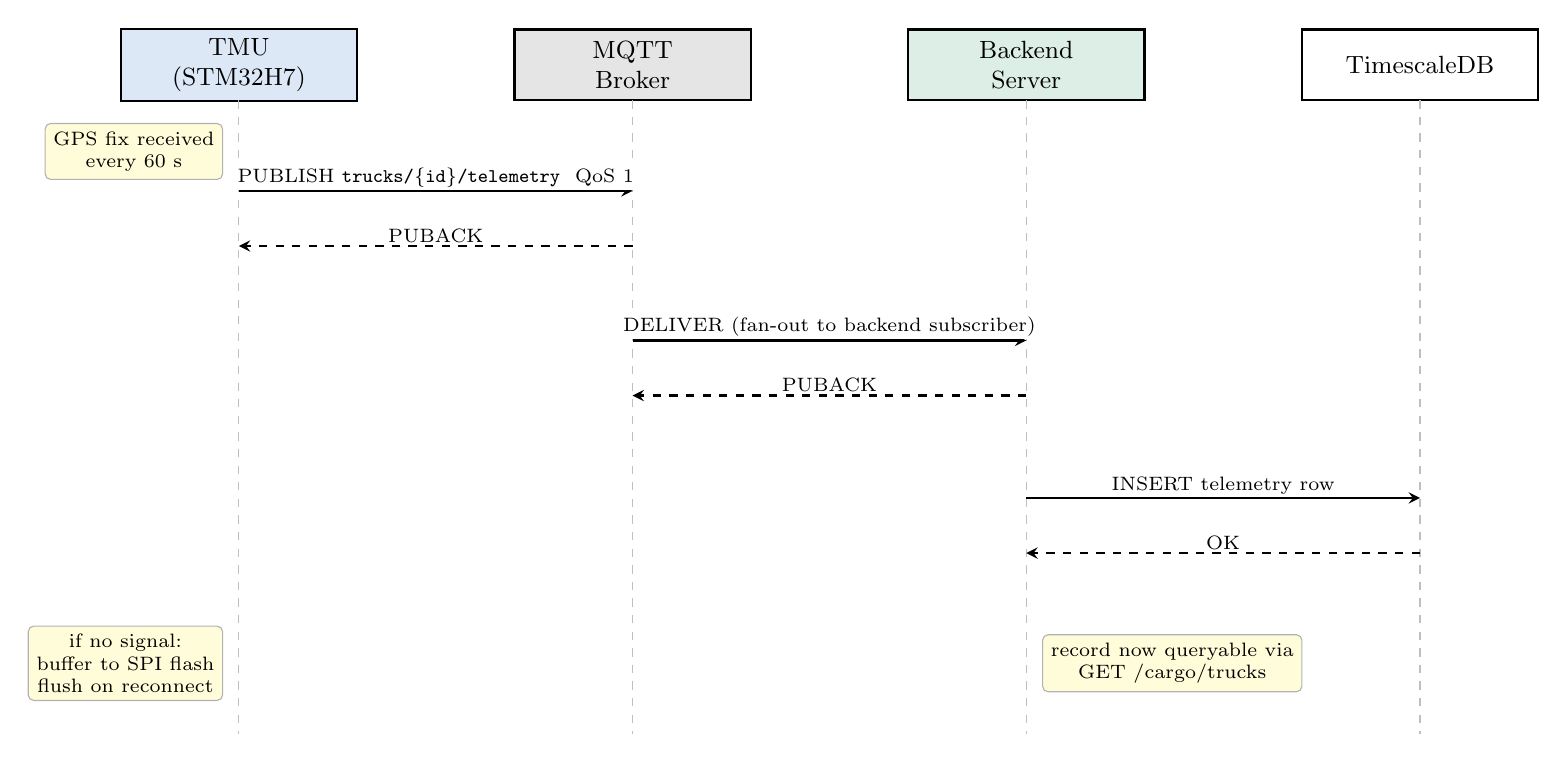
\begin{tikzpicture}[
    actor/.style={rectangle, draw, thick, minimum width=3.0cm, minimum height=0.9cm,
                  text centered, align=center, font=\small},
    msg/.style={->, thick, >=stealth},
    ret/.style={->, thick, dashed, >=stealth},
    lbl/.style={font=\scriptsize, fill=white, inner sep=1pt},
    ann/.style={draw=gray!60, rounded corners=2pt, fill=yellow!15,
                font=\scriptsize, inner sep=3pt, align=center}]

%% Actor headers
\node[actor, fill=evblue!15]   at (0,0)  {TMU\\(STM32H7)};
\node[actor, fill=gray!20]     at (5,0)  {MQTT\\Broker};
\node[actor, fill=emsgreen!15] at (10,0) {Backend\\Server};
\node[actor]                   at (15,0) {TimescaleDB};

%% Lifelines
\foreach \x in {0,5,10,15}
    \draw[dashed, gray!50] (\x,-0.45) -- (\x,-8.5);

%% Trigger annotation
\node[ann, anchor=east] at (-0.2,-1.1) {GPS fix received\\every 60 s};

%% 1. PUBLISH
\draw[msg] (0,-1.6) -- node[lbl,above]{PUBLISH \texttt{trucks/\{id\}/telemetry}~~QoS 1} (5,-1.6);

%% 2. PUBACK
\draw[ret] (5,-2.3) -- node[lbl,above]{PUBACK} (0,-2.3);

%% 3. DELIVER
\draw[msg] (5,-3.5) -- node[lbl,above]{DELIVER (fan-out to backend subscriber)} (10,-3.5);

%% 4. PUBACK from backend
\draw[ret] (10,-4.2) -- node[lbl,above]{PUBACK} (5,-4.2);

%% 5. INSERT into DB
\draw[msg] (10,-5.5) -- node[lbl,above]{INSERT telemetry row} (15,-5.5);

%% 6. OK
\draw[ret] (15,-6.2) -- node[lbl,above]{OK} (10,-6.2);

%% Result note
\node[ann, anchor=west] at (10.2,-7.6)
    {record now queryable via\\GET /cargo/trucks};

%% If offline: buffer annotation
\node[ann, anchor=east] at (-0.2,-7.6)
    {if no signal:\\buffer to SPI flash\\flush on reconnect};

\end{tikzpicture}%
}
\caption{Telemetry upload sequence. QoS~1 ensures the broker stores the
message until the backend acknowledges. Offline messages are buffered locally
and flushed (5 records/s) once connectivity returns.}
\label{fig:telemetry-flow}
\end{figure}

% ==============================================================================
\section{Station Departure Trigger and Photo Upload}
\label{sec:photo-flow}
% ==============================================================================

\subsection{Geo-Fence Logic}
\label{sec:geofence}

The TMU implements a per-station geo-fence state machine. Station coordinates are
downloaded from the server at startup (see Section~\ref{sec:bootstrap}) and
stored in flash.

\textbf{Departure is declared} when the truck's GPS position crosses
\textbf{200 metres} from the station centre, \emph{after} having been inside the
radius. This prevents a false trigger when the truck passes near a station without
stopping.

\begin{figure}[h]
\centering
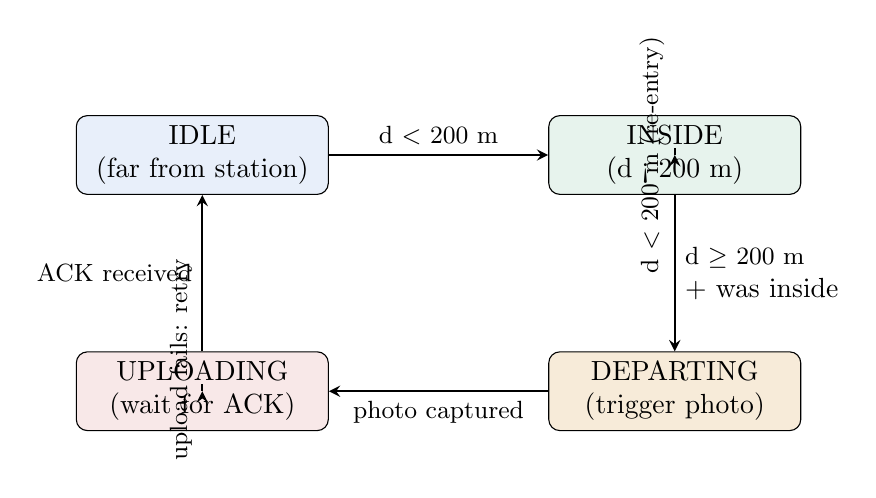
\begin{tikzpicture}[
    state/.style={rectangle, rounded corners, draw, minimum width=3.2cm,
                  minimum height=1cm, text centered, align=center, fill=gray!10},
    arrow/.style={thick,->,>=stealth}]

\node (idle)     [state, fill=evblue!10]     at (0,0)    {IDLE\\(far from station)};
\node (inside)   [state, fill=emsgreen!10]   at (6,0)    {INSIDE\\(d < 200 m)};
\node (depart)   [state, fill=cargoamber!15] at (6,-3)   {DEPARTING\\(trigger photo)};
\node (uploading)[state, fill=stmred!10]     at (0,-3)   {UPLOADING\\(wait for ACK)};

\draw [arrow] (idle)   -- node[above]{\small d $<$ 200 m} (inside);
\draw [arrow] (inside) -- node[right, align=left]{\small d $\geq$ 200 m\\+ was inside} (depart);
\draw [arrow] (depart) -- node[below]{\small photo captured} (uploading);
\draw [arrow] (uploading) -- node[left]{\small ACK received} (idle);
\draw [arrow] (inside) to[bend left=25] node[above, sloped]{\small d $<$ 200 m (re-entry)} (inside);
\draw [arrow] (uploading) to[bend right=30]
    node[above, sloped, xshift=4mm]{\small upload fails: retry} (uploading);
\end{tikzpicture}
\caption{Station departure geo-fence state machine}
\end{figure}

\subsection{Haversine Distance Calculation}

The TMU computes the great-circle distance from the current GPS fix to the
station centre using the Haversine formula. This is cheap enough to run on the
STM32H7 every GPS fix (once per second while moving).

\begin{equation}
d = 2R \arcsin\!\left(\sqrt{
    \sin^2\!\left(\frac{\phi_2 - \phi_1}{2}\right)
    + \cos\phi_1\cos\phi_2\sin^2\!\left(\frac{\lambda_2 - \lambda_1}{2}\right)
}\right)
\end{equation}

where $R = 6{,}371{,}000$ m, $\phi$ = latitude in radians,
$\lambda$ = longitude in radians.

\begin{lstlisting}[language=c, caption=Haversine in C (STM32H7)]
#include <math.h>
#define EARTH_R_M  6371000.0f

float haversine_m(float lat1, float lon1, float lat2, float lon2) {
    float dlat = (lat2 - lat1) * M_PI / 180.0f;
    float dlon = (lon2 - lon1) * M_PI / 180.0f;
    float a = sinf(dlat / 2) * sinf(dlat / 2)
            + cosf(lat1 * M_PI / 180.0f)
            * cosf(lat2 * M_PI / 180.0f)
            * sinf(dlon / 2) * sinf(dlon / 2);
    return 2.0f * EARTH_R_M * asinf(sqrtf(a));
}
\end{lstlisting}

\subsection{Step-by-Step Departure Flow}

\begin{enumerate}[leftmargin=*, label=\textbf{Step \arabic*.}]

    \item \textbf{Transition to DEPARTING.}
    When \texttt{haversine\_m()} returns $\geq 200$ m and the state was
    \texttt{INSIDE}, the TMU transitions to \texttt{DEPARTING} and immediately:
    \begin{itemize}
        \item Records \texttt{departureTs} (GPS timestamp).
        \item Records the last GPS fix inside the station (\texttt{lastInsideFix}).
        \item Publishes a departure event to \texttt{trucks/\{id\}/event}.
    \end{itemize}

    \begin{lstlisting}[language=json, caption=Departure event payload]
{
  "v":         1,
  "type":      "StationDeparture",
  "ts":        1751501100,
  "stationId": "site-bkk-001",
  "loadPct":   85,           // from load sensor at time of departure
  "gps": {
    "lat": 13.7302, "lng": 100.7541,
    "speedKph": 22, "headingDeg": 112
  }
}
    \end{lstlisting}

    \item \textbf{Fetch snapshot from IP camera.}
    Immediately after publishing the departure event the TMU sends an HTTP GET
    to each camera's snapshot endpoint on the truck LAN:
    \begin{lstlisting}[language=bash, caption=Camera snapshot fetch (on-board LAN)]
GET http://192.168.1.11/snapshot.jpg     # Camera 1 -- cargo front (SPI-Eth 1)
GET http://192.168.2.11/snapshot.jpg     # Camera 2 -- cargo rear  (SPI-Eth 2)
Timeout: 5 s per camera
    \end{lstlisting}
    The cameras return a JPEG directly. No video stream is opened. If the
    camera does not respond within 5 s, the TMU retries once, then proceeds
    without that camera's photo and logs \texttt{cameraError: true}.
    \begin{itemize}
        \item Expected resolution from camera: $1920 \times 1080$ or
              $1280 \times 960$ px (camera-dependent).
        \item If the raw JPEG exceeds 512 KB, the TMU re-encodes it at reduced
              JPEG quality (try 70, then 55) using the STM32H7 JPEG hardware
              encoder until the file fits.
        \item The TMU writes the GPS timestamp and \texttt{truckId} into the
              EXIF \texttt{UserComment} field before upload (preserving
              the original camera EXIF otherwise).
    \end{itemize}

    \item \textbf{Upload via HTTPS POST.}
    The TMU posts each JPEG to the fixed backend endpoint
    \texttt{POST /v1/trucks/\{id\}/photos} with context headers
    (\texttt{X-Station-Id}, \texttt{X-Camera}, \texttt{X-Timestamp}).
    The server stores the image and responds \texttt{200 OK} with a
    JSON body containing the assigned \texttt{photoId}.
    The two cameras upload independently; if one fails, the other proceeds.

    \item \textbf{Publish photo-ready notification.}
    After each successful upload the TMU publishes to
    \texttt{trucks/\{id\}/photo/ready}:

    \begin{lstlisting}[language=json, caption=PhotoReady notification (one per camera)]
{
  "v":         1,
  "photoId":   "photo-0041-001",   // assigned by server in upload response
  "stationId": "site-bkk-001",
  "camera":    "cargo-front",      // cargo-front | cargo-rear
  "ts":        1751501135,
  "fileSizeKb": 342,
  "loadPct":    85,
  "cameraError": false             // true if snapshot fetch failed
}
    \end{lstlisting}

    \noindent Both cameras upload independently and each sends its own
    \texttt{PhotoReady} event. The backend links both records under
    \texttt{cargoPhotos: [ \{camera: "cargo-front", ...\},
    \{camera: "cargo-rear", ...\} ]} and emits a \texttt{CargoPhotoReady}
    WebSocket event to the dashboard.

    \item \textbf{Transition to IDLE.}
    On receipt of the server ACK (or after a 30 s timeout) the TMU returns to
    \texttt{IDLE} and the station departure cycle is complete.

\end{enumerate}

\subsection{Error and Retry Handling}

\begin{center}
\begin{tabular}{lll}
\toprule
\textbf{Failure} & \textbf{TMU action} & \textbf{Max attempts}\\
\midrule
No URL received in 10 s    & Re-publish departure event & 3 $\times$ (then log and skip)\\
HTTPS PUT timeout / 5xx    & Retry with exponential backoff (2 s, 4 s, 8 s) & 3\\
HTTPS PUT 4xx (URL expired)& Re-request URL via departure event & 2\\
Camera capture failure     & Log fault, publish event with \texttt{photoError: true} & ---\\
\bottomrule
\end{tabular}
\end{center}

If all retries are exhausted the TMU publishes a \texttt{PhotoFailed} event and
transitions to \texttt{IDLE}. The trip record on the server will have
\texttt{cargoPhoto: null} with a \texttt{photoError} reason field.

\subsection{Photo Upload Flow}

\begin{figure}[h]
\centering
\resizebox{\textwidth}{!}{%
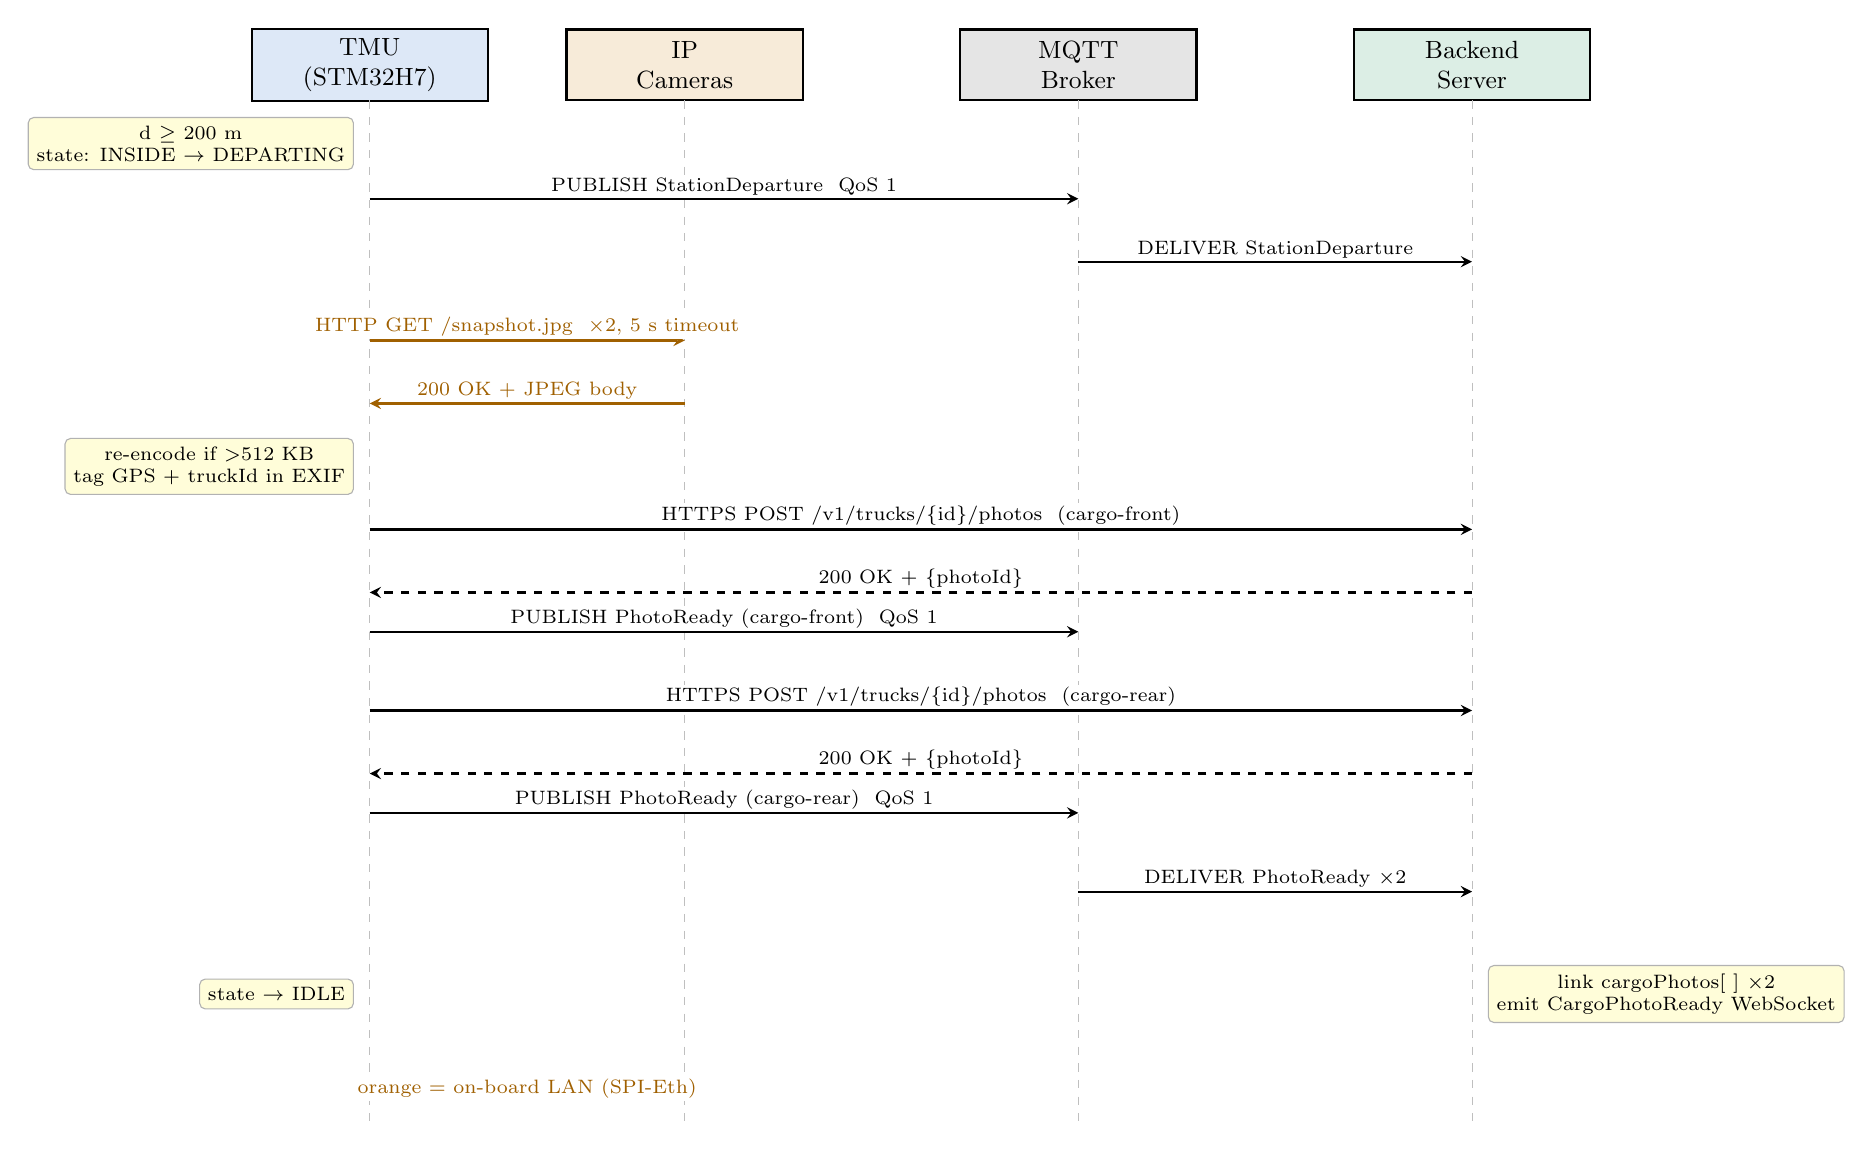
\begin{tikzpicture}[
    actor/.style={rectangle, draw, thick, minimum width=3.0cm, minimum height=0.9cm,
                  text centered, align=center, font=\small},
    msg/.style={->, thick, >=stealth},
    ret/.style={->, thick, dashed, >=stealth},
    lan/.style={->, thick, >=stealth, cargoamber!80!black},
    lbl/.style={font=\scriptsize, fill=white, inner sep=1pt},
    ann/.style={draw=gray!60, rounded corners=2pt, fill=yellow!15,
                font=\scriptsize, inner sep=3pt, align=center}]

%% Actors: TMU=0, Cameras=4, Broker=9, Backend=14
\node[actor, fill=evblue!15]     at (0,0)  {TMU\\(STM32H7)};
\node[actor, fill=cargoamber!15] at (4,0)  {IP\\Cameras};
\node[actor, fill=gray!20]       at (9,0)  {MQTT\\Broker};
\node[actor, fill=emsgreen!15]   at (14,0) {Backend\\Server};

%% Lifelines
\foreach \x in {0,4,9,14}
    \draw[dashed, gray!50] (\x,-0.45) -- (\x,-13.5);

%% ── Trigger ──────────────────────────────────────────────────────────
\node[ann, anchor=east] at (-0.2,-1.0)
    {d $\geq$ 200 m\\state: INSIDE $\to$ DEPARTING};

%% 1. Publish departure
\draw[msg] (0,-1.7) -- node[lbl,above]{PUBLISH StationDeparture~~QoS 1} (9,-1.7);

%% 2. Deliver to backend
\draw[msg] (9,-2.5) -- node[lbl,above]{DELIVER StationDeparture} (14,-2.5);

%% ── Camera capture (on-board LAN, orange) ────────────────────────────
%% 3. HTTP GET snapshot ×2
\draw[lan] (0,-3.5) -- node[lbl,above]{\textcolor{cargoamber!80!black}{HTTP GET /snapshot.jpg~~$\times 2$, 5 s timeout}} (4,-3.5);

%% 4. 200 OK + JPEG body
\draw[lan] (4,-4.3) -- node[lbl,above]{\textcolor{cargoamber!80!black}{200 OK + JPEG body}} (0,-4.3);

%% 5. Re-encode annotation
\node[ann, anchor=east] at (-0.2,-5.1)
    {re-encode if $>$512 KB\\tag GPS + truckId in EXIF};

%% ── Direct upload to backend (cargo-front) ───────────────────────────
%% 6. HTTPS POST front
\draw[msg] (0,-5.9) -- node[lbl,above]{HTTPS POST /v1/trucks/\{id\}/photos~~(cargo-front)} (14,-5.9);

%% 7. 200 OK + photoId
\draw[ret] (14,-6.7) -- node[lbl,above]{200 OK + \{photoId\}} (0,-6.7);

%% 8. PhotoReady front
\draw[msg] (0,-7.2) -- node[lbl,above]{PUBLISH PhotoReady (cargo-front)~~QoS 1} (9,-7.2);

%% ── Direct upload to backend (cargo-rear) ────────────────────────────
%% 9. HTTPS POST rear
\draw[msg] (0,-8.2) -- node[lbl,above]{HTTPS POST /v1/trucks/\{id\}/photos~~(cargo-rear)} (14,-8.2);

%% 10. 200 OK + photoId
\draw[ret] (14,-9.0) -- node[lbl,above]{200 OK + \{photoId\}} (0,-9.0);

%% 11. PhotoReady rear
\draw[msg] (0,-9.5) -- node[lbl,above]{PUBLISH PhotoReady (cargo-rear)~~QoS 1} (9,-9.5);

%% ── Backend receives PhotoReady ×2 ───────────────────────────────────
%% 12. Deliver PhotoReady ×2
\draw[msg] (9,-10.5) -- node[lbl,above]{DELIVER PhotoReady $\times 2$} (14,-10.5);

%% 13. Annotations
\node[ann, anchor=west] at (14.2,-11.8)
    {link cargoPhotos[ ] $\times 2$\\emit CargoPhotoReady WebSocket};

\node[ann, anchor=east] at (-0.2,-11.8)
    {state $\to$ IDLE};

%% Legend
\node[lbl, text=cargoamber!80!black] at (2,-13.0)
    {orange = on-board LAN (SPI-Eth)};

\end{tikzpicture}%
}
\caption{Photo upload sequence. Orange: on-board LAN between TMU and cameras
(HTTP over SPI-Ethernet, never leaves the truck). Black solid: MQTT events.
Black dashed: HTTPS responses. The truck uploads directly to the backend
at a fixed endpoint --- no URL is exchanged via the broker.}
\label{fig:photo-flow}
\end{figure}

% ==============================================================================
\section{Offline Buffering}
\label{sec:buffer}
% ==============================================================================

When the modem loses signal, telemetry must not be silently dropped. The TMU
writes unsent records to a FIFO ring buffer in internal or external flash.

\begin{center}
\begin{tabular}{ll}
\toprule
\textbf{Parameter} & \textbf{Value}\\
\midrule
Buffer medium        & External SPI NOR flash (or STM32H7 internal flash sector)\\
Record size          & $\leq 256$ bytes (one telemetry JSON, compressed if needed)\\
Buffer capacity      & 512 records ($\approx$ 8.5 hours at 60 s interval)\\
Flush order          & FIFO --- oldest records published first on reconnect\\
Max flush rate       & 5 records/s (avoid broker overload on long reconnect)\\
Buffer overflow      & Overwrite oldest records; increment \texttt{droppedCount} counter\\
\bottomrule
\end{tabular}
\end{center}

The \texttt{device.bufferDepth} field in each telemetry message tells the server
how many records are still queued on the device. The \texttt{device.seqNo}
counter allows the server to detect any records that were overwritten and
mark them as missing in the trip log.

% ==============================================================================
\section{Connection Management}
% ==============================================================================

\subsection{Reconnect Strategy}

\begin{lstlisting}[language=c, caption=Reconnect backoff (pseudocode)]
uint32_t backoff_ms = 1000;
const uint32_t MAX_BACKOFF_MS = 60000;

while (!mqtt_connected()) {
    if (mqtt_connect() == MQTT_OK) {
        backoff_ms = 1000;   // reset on success
        flush_buffer();
        break;
    }
    os_delay(backoff_ms);
    backoff_ms = MIN(backoff_ms * 2, MAX_BACKOFF_MS);
}
\end{lstlisting}

\subsection{MQTT Last Will and Testament}

The TMU registers a Last Will message at connect time. The broker publishes it
automatically if the client disconnects without sending DISCONNECT:

\begin{lstlisting}[language=json, caption=Last Will payload]
{
  "v":     1,
  "type":  "DeviceOffline",
  "ts":    0,          // broker fills this with its own timestamp
  "truckId": "truck-bkk-007"
}
\end{lstlisting}

Topic: \texttt{trucks/\{id\}/event}, QoS 1, Retain: \texttt{false}.

The server marks the truck as \texttt{Offline} in the dashboard when this
message is received.

\subsection{Heartbeat}

The MQTT keep-alive (60 s) acts as the heartbeat. No separate application-level
ping is required. If the broker does not receive any packet (PUBLISH, PINGREQ,
etc.) within 1.5 $\times$ keep-alive = 90 s, it closes the connection and
triggers the Last Will.

% ==============================================================================
\section{Server-to-Device Commands}
% ==============================================================================

The server may send commands to the TMU on \texttt{trucks/\{id\}/cmd}.
The TMU must acknowledge every command within 10 s.

\begin{lstlisting}[language=json, caption=Command envelope]
{
  "v":       1,
  "cmdId":   "cmd-20260702-0099",
  "type":    "CapturePhoto",          // see table below
  "payload": { }
}
\end{lstlisting}

\begin{center}
\begin{tabular}{lll}
\toprule
\textbf{type} & \textbf{payload fields} & \textbf{Action}\\
\midrule
\texttt{CapturePhoto}   & \texttt{camera} (\texttt{cargo}|\texttt{road}) & Capture and upload immediately\\
\texttt{UpdateStations} & \texttt{stations} (array of Station objects)   & Reload geo-fence table\\
\texttt{SetInterval}    & \texttt{intervalSec} (30--300)                 & Change telemetry interval\\
\texttt{Reboot}         & ---                                            & Soft-reboot MCU\\
\texttt{FirmwareUpdate} & \texttt{url}, \texttt{sha256}                  & OTA firmware download\\
\bottomrule
\end{tabular}
\end{center}

\textbf{Acknowledgement} published to \texttt{trucks/\{id\}/event}:

\begin{lstlisting}[language=json, caption=Command acknowledgement]
{
  "v":     1,
  "type":  "CmdAck",
  "cmdId": "cmd-20260702-0099",
  "ts":    1751501200,
  "status": "OK"            // OK | Error
}
\end{lstlisting}

% ==============================================================================
\section{Bootstrap and Station Table}
\label{sec:bootstrap}
% ==============================================================================

On first boot (or after a firmware update) the TMU has no station coordinates.
It must request them before the geo-fence logic can operate.

\begin{enumerate}[leftmargin=*, label=\textbf{Step \arabic*.}]
    \item TMU connects to MQTT broker.
    \item TMU publishes a \texttt{Bootstrap} event to \texttt{trucks/\{id\}/event}:
    \begin{lstlisting}[language=json]
{ "v": 1, "type": "Bootstrap", "ts": 1751500000,
  "firmware": "1.4.2", "stationTableVersion": 0 }
    \end{lstlisting}
    \item Server responds with \texttt{UpdateStations} command containing the
          full station table (id, name, lat, lng for every station on the
          truck's assigned routes).
    \item TMU stores the table in flash, sets \texttt{stationTableVersion}
          to the version field in the payload, and enters normal operation.
    \item The server re-sends \texttt{UpdateStations} whenever the route
          assignment changes. The TMU checks the version on every boot and
          requests a refresh if its stored version is stale.
\end{enumerate}

\subsubsection*{UpdateStations payload --- station array}

Each element in \texttt{payload.stations} is a static reference record
containing the fields the TMU needs to run the geo-fence state machine.
The geo-fence circle for each station is fully defined by its
\texttt{lat}/\texttt{lng} centre and the protocol-constant 200 m radius
(Section~\ref{sec:geofence}). \texttt{name} is stored for diagnostic
logs only. The \texttt{version} field lets the TMU detect a stale cache
on reboot.

\begin{lstlisting}[language=json, caption=Topic: trucks/truck-bkk-007/cmd | QoS 1 (server $\to$ truck)]
{
  "v":      1,
  "cmdId":  "cmd-bootstrap-001",
  "type":   "UpdateStations",
  "payload": {
    "version": 7,
    "stations": [
      {
        "id":   "site-bkk-001",
        "name": "Lad Krabang Hub",
        "lat":  13.7284,
        "lng":  100.7498
      },
      {
        "id":   "site-bkk-002",
        "name": "Don Mueang Depot",
        "lat":  13.9125,
        "lng":  100.6068
      },
      {
        "id":   "site-bkk-003",
        "name": "Samut Prakan Cold Hub",
        "lat":  13.5991,
        "lng":  100.5975
      },
      {
        "id":   "site-bkk-004",
        "name": "Bang Na Distribution Centre",
        "lat":  13.6623,
        "lng":  100.6501
      }
    ]
  }
}
\end{lstlisting}

\noindent On every GPS fix the TMU calls \texttt{haversine\_m()} against
each entry. A station whose distance falls below 200 m triggers the
\texttt{INSIDE} transition for that geo-fence.

% ==============================================================================
\section{Bandwidth Budget}
% ==============================================================================

\begin{center}
\begin{tabular}{lrrr}
\toprule
\textbf{Message type} & \textbf{Size} & \textbf{Frequency} & \textbf{Per hour}\\
\midrule
Telemetry (GPS + OBD) & $\approx 350$ B & 1/min & $\approx 21$ KB\\
Departure event       & $\approx 200$ B & 2--6/day & $<$ 1 KB\\
Photo upload (JPEG)   & $\leq 512$ KB   & 2--6/day & $\leq 3$ MB\\
MQTT keep-alive ping  & 2 B             & 1/min    & $< 1$ KB\\
\midrule
\textbf{Daily total (typical)} & & & $\approx$ \textbf{25--40 MB}\\
\bottomrule
\end{tabular}
\end{center}

\noindent A standard 3G/4G data plan of \textbf{1 GB/month per truck} provides
more than sufficient headroom. The dominant cost is photo uploads, not telemetry.

% ==============================================================================
\section{Summary of MQTT Topics}
% ==============================================================================

\begin{longtable}{>{\ttfamily\small}p{0.46\textwidth} p{0.08\textwidth} p{0.36\textwidth}}
\toprule
\textbf{Topic} & \textbf{QoS} & \textbf{Description}\\
\midrule
\endfirsthead
\toprule
\textbf{Topic} & \textbf{QoS} & \textbf{Description}\\
\midrule
\endhead
\bottomrule
\endfoot
trucks/\{id\}/telemetry   & 1 & GPS + OBD-II payload, every 60 s\\
trucks/\{id\}/event       & 1 & StationDeparture, Bootstrap, CmdAck, DeviceOffline\\
trucks/\{id\}/photo/ready & 1 & Notify server photo upload complete (one per camera)\\
trucks/\{id\}/cmd         & 1 & Server-to-device command\\
\end{longtable}

% ==============================================================================
\section{Message Examples}
\label{sec:msg-examples}
% ==============================================================================

The examples below use truck ID \texttt{truck-bkk-007}. All timestamps are
UTC Unix seconds. Arrow direction shows who publishes the message.

% ------------------------------------------------------------------------------
\subsection{Device Lifecycle}

\textbf{DeviceOnline} --- truck $\to$ server, published on every MQTT connect:

\begin{lstlisting}[language=json, caption=Topic: trucks/truck-bkk-007/event | QoS 1]
{
  "v":       1,
  "type":    "DeviceOnline",
  "ts":      1751500800,
  "clkSource": "GPS",
  "firmware": "1.4.2",
  "stationTableVersion": 7
}
\end{lstlisting}

\textbf{DeviceOffline} --- auto-published by the \emph{broker} via Last Will
when the TCP connection drops without a clean disconnect:

\begin{lstlisting}[language=json, caption=Topic: trucks/truck-bkk-007/event | QoS 1 | retain: true]
{
  "v":    1,
  "type": "DeviceOffline",
  "ts":   0
}
\end{lstlisting}

\noindent The \texttt{ts: 0} is the Last Will payload set at connect time;
the server records the broker receive timestamp instead.

% ------------------------------------------------------------------------------
\subsection{60-Second Telemetry}

\textbf{Telemetry} --- truck $\to$ server, once per minute while ignition on:

\begin{lstlisting}[language=json, caption=Topic: trucks/truck-bkk-007/telemetry | QoS 1]
{
  "v":   1,
  "ts":  1751500860,
  "gps": {
    "lat":        13.8562,
    "lng":        100.6211,
    "altM":       12.5,
    "speedKph":   68.2,
    "headingDeg": 245,
    "hdop":       1.2,
    "satellites": 8,
    "fixType":    "3D"
  },
  "obd": {
    "speedKph":     68,
    "rpm":          2100,
    "engineLoadPct":42,
    "coolantTempC": 89,
    "fuelLevelPct": 67,
    "throttlePct":  35,
    "dtcCount":     0,
    "mil":          false
  },
  "device": {
    "battV":      12.8,
    "signalDbm":  -82,
    "seqNo":      1247,
    "bufferDepth":0,
    "clkSource":  "GPS"
  }
}
\end{lstlisting}

% ------------------------------------------------------------------------------
\subsection{Station Visit}

\textbf{StationArrival} --- truck $\to$ server, fired when geo-fence state
transitions to \texttt{INSIDE} (distance $<$ 200 m):

\begin{lstlisting}[language=json, caption=Topic: trucks/truck-bkk-007/event | QoS 1]
{
  "v":        1,
  "type":     "StationArrival",
  "ts":       1751501100,
  "stationId":"site-bkk-001",
  "distM":    145.3,
  "tripId":   "trip-20260702-0041"
}
\end{lstlisting}

\textbf{StationDeparture} --- truck $\to$ server, fired when geo-fence state
transitions to \texttt{DEPARTING} (distance $\geq$ 200 m after being inside).
This is also the trigger for the photo upload flow:

\begin{lstlisting}[language=json, caption=Topic: trucks/truck-bkk-007/event | QoS 1]
{
  "v":        1,
  "type":     "StationDeparture",
  "ts":       1751503200,
  "stationId":"site-bkk-001",
  "distM":    201.8,
  "loadPct":  85,
  "tripId":   "trip-20260702-0041"
}
\end{lstlisting}

\textbf{Photo upload} --- truck $\to$ backend, one HTTPS POST per camera
to the fixed upload endpoint (no URL exchange required):

\begin{lstlisting}[language=bash, caption=HTTPS POST photo upload (repeated for cargo-rear)]
POST http://91.210.146.166:3000/v1/trucks/truck-bkk-007/photos
Content-Type: image/jpeg
X-Station-Id: site-bkk-001
X-Camera:     cargo-front
X-Timestamp:  1751503201
<binary JPEG body, max 512 KB>

// Response 200 OK:
{ "photoId": "photo-0041-001" }
\end{lstlisting}

\textbf{PhotoReady} --- truck $\to$ server, after HTTPS POST succeeds for each
camera. The \texttt{photoId} was returned by the upload response and lets
the backend correlate the MQTT event with the stored image:

\begin{lstlisting}[language=json, caption=Topic: trucks/truck-bkk-007/photo/ready | QoS 1]
{
  "v":         1,
  "type":      "PhotoReady",
  "ts":        1751503245,
  "photoId":   "photo-0041-001",
  "camera":    "cargo-front",
  "stationId": "site-bkk-001",
  "sizeBytes": 398420,
  "cameraError": false
}
\end{lstlisting}

% ------------------------------------------------------------------------------
\subsection{Server Commands}

\textbf{SetInterval command} --- server $\to$ truck, changing the telemetry
publish interval:

\begin{lstlisting}[language=json, caption=Topic: trucks/truck-bkk-007/cmd | QoS 1]
{
  "v":      1,
  "cmdId":  "cmd-20260702-0099",
  "type":   "SetInterval",
  "payload":{ "intervalSec": 30 }
}
\end{lstlisting}

\textbf{CmdAck} --- truck $\to$ server, within 10 s of receiving the command:

\begin{lstlisting}[language=json, caption=Topic: trucks/truck-bkk-007/event | QoS 1]
{
  "v":     1,
  "type":  "CmdAck",
  "cmdId": "cmd-20260702-0099",
  "ts":    1751501200,
  "status":"OK"
}
\end{lstlisting}

\textbf{FirmwareUpdate command} --- server $\to$ truck, triggering an OTA
download. The truck fetches the binary via HTTPS, verifies the SHA-256 hash,
writes to flash, and reboots:

\begin{lstlisting}[language=json, caption=Topic: trucks/truck-bkk-007/cmd | QoS 1]
{
  "v":      1,
  "cmdId":  "cmd-20260702-0100",
  "type":   "FirmwareUpdate",
  "payload":{
    "version": "1.5.0",
    "url":     "http://91.210.146.166:3000/firmware/tmu-1.5.0.bin",
    "sha256":  "a3f5e2...c9d1"
  }
}
\end{lstlisting}

\end{document}
